\documentclass[a4paper,12pt]{article}
\usepackage[polish]{babel}
\usepackage[utf8]{inputenc}
\usepackage{graphicx}
\usepackage{amsmath}
\usepackage{hyperref}
\usepackage{geometry}
\usepackage[T1]{fontenc}
\usepackage{lmodern}
\usepackage{listings}
\usepackage{siunitx}
\usepackage{listings}
\usepackage{float}

\geometry{margin=1in}

\setcounter{secnumdepth}{4}
\setcounter{tocdepth}{4}

\lstset{
  literate={ą}{{\k a}}1
  		     {Ą}{{\k A}}1
           {ż}{{\. z}}1
           {Ż}{{\. Z}}1
           {ź}{{\' z}}1
           {Ź}{{\' Z}}1
           {ć}{{\' c}}1
           {Ć}{{\' C}}1
           {ę}{{\k e}}1
           {Ę}{{\k E}}1
           {ó}{{\' o}}1
           {Ó}{{\' O}}1
           {ń}{{\' n}}1
           {Ń}{{\' N}}1
           {ś}{{\' s}}1
           {Ś}{{\' S}}1
           {ł}{{\l}}1
           {Ł}{{\L}}1
}
\usepackage{xcolor}

\definecolor{codebg}{rgb}{0.95,0.95,0.95} % Kolor tła dla listingu
\definecolor{string}{rgb}{0.58,0,0.82}    % Kolor dla stringów
\definecolor{keyword}{rgb}{0,0,0.8}       % Kolor dla słów kluczowych
\definecolor{comment}{rgb}{0,0.5,0}       % Kolor dla komentarzy

\lstset{
    float,
    language=C,
    backgroundcolor=\color{codebg},
    basicstyle=\ttfamily\small,
    keywordstyle=\color{keyword}\bfseries,
    stringstyle=\color{string},
    commentstyle=\color{comment}\itshape,
    numbers=left,
    numberstyle=\tiny\color{gray},
    stepnumber=1,
    numbersep=10pt,
    frame=single,
    rulecolor=\color{black},
    tabsize=4,
    showstringspaces=false,
    breaklines=true,
    breakatwhitespace=true,
    captionpos=b,
    escapeinside={(*@}{@*)} % Pozwala na wstawianie elementów LaTeX w listingu
}

\title{
    \textbf{Sprawozdanie} \\
    Zastosowanie MPI oraz OpenMP w procesie generowania skrótów MD5 dla kolejnych kombinacji zbioru znaków \\
    \small Programowanie Równoległe i Rozproszone
}
\author{Łukasz Niedzielski, Dominik Madej}
\date{15 stycznia 2025}

\begin{document}

\maketitle{}

\tableofcontents{}

\newpage

\section{Wprowadzenie}
Celem pracy było zaimplementowanie i analiza algorytmu obliczania i porównywania skrótów MD5 dla kolejnych kombinacji znaków o ustalonej długości z podanego alfabetu. Jednym z zastosowań tego algorytmu jest łamanie haseł poprzez szukanie wiadomości, której skrót jest taki sam jak szukanego hasła. W sprawozdaniu opisano implementację algorytmu w wersji sekwencyjnej oraz równoległej (z wykorzystaniem OpenMP, MPI oraz kombinacji MPI+OpenMP). Przedstawiono także uzyskane wyniki w postaci wykresów oraz omówiono wpływ zastosowanych metod zrównoleglenia na wydajność programu.

\section{Opis algorytmu}
Algorytm polega na:
\begin{enumerate}
	\item Generowaniu kolejnych kombinacji bez powtórzeń znaków o określonej długości z ustalonego alfabetu.
	\item Obliczaniu skrótu MD5 dla każdej kombinacji.
	\item Porównywaniu uzyskanego skrótu z poszukiwanym skrótem.
	\item Zakończeniu działania programu po znalezieniu pasującej kombinacji lub po sprawdzeniu określonej liczby kombinacji.
\end{enumerate}
Dane wejściowe algorytmu to:
\begin{itemize}
	\item Długość wiadomości (np. 8 znaków),
	\item Alfabet (np. \texttt{abcdefghijklmnopqrstuvwxyz}),
	\item Skrót MD5 poszukiwanej wiadomości (np. \texttt{9e65ff77204283d4a951e12d2bb8357e}),
	\item Liczba wiadomości do sprawdzenia (np. $2^{24}$).
\end{itemize}
Dane wyjściowe to znaleziona wiadomość lub informacja o jej braku.

\subsection{Generowanie kolejnych kombinacji bez powtórzeń}

Sposób generowania kolejnych kombinacji znaków opiera się na reprezentacji pozycyjnej (podobnej do systemu liczbowego). Każdy znak w kombinacji jest traktowany jako ``cyfra'', a alfabet jako ``podstawa'' tego systemu. Iterując przez wszystkie możliwe liczby w takim systemie, generujemy kombinacje w sposób deterministyczny i przewidywalny. Dzięki temu można w prosty sposób podzielić zakres kombinacji między różne wątki lub procesy, co jest kluczowe w implementacji równoległej.

Możliwość zastosowania tego sposobu wynika z jego deterministycznej natury, która gwarantuje wygenerowanie wszystkich możliwych kombinacji przy minimalnym narzucie obliczeniowym. Dodatkowo reprezentacja pozycyjna pozwala na łatwe przeliczanie zakresów kombinacji w środowiskach równoległych, co znacznie upraszcza implementację zrównoleglenia algorytmu.

\section{Implementacja algorytmu}

Przygotowane implementacje korzystają z poniższej procedury w celu sprawdzenia \lstinline{hashes_to_check} kolejnych kombinacji, zaczynając od kombinacji o numerze \lstinline{combination_number}.

\begin{figure}[H]
	\begin{lstlisting}[caption={Sprawdzanie partii wiadomości.}]
struct search_result check_batch(size_t combination_number, size_t length, size_t hashes_to_check, uint8_t orginal_hash[16]) {
    char *password = NULL;
    size_t indices[PASSWORD_LENGTH] = {};
    get_nth_combinaiton(indices, combination_number, length);

    int pos = length - 1;
    char buffer[PASSWORD_LENGTH + 1] = {0};
    uint8_t result[16];

    size_t checked_hashes = 0;
    while (checked_hashes < hashes_to_check && pos >= 0) {
        // ustawienie kolejnej kombinacji z powtórzeniami
        next_combination(buffer, indices, &pos);

        // wyznaczenie skrótu kombinacji
        md5String(buffer, length, result);
        checked_hashes++;

        // sprawdzanie czy skróty się zgadzają
        if (memcmp(orginal_hash, result, 16) == 0) {
            // znaleziono pasuąjącą wiadomość - koniec algorytmu
            password = clone(buffer);
            break;
        }
        // czyszczenie wiadomosci
        memset(buffer, 0, PASSWORD_LENGTH);
    }

    struct search_result search_result = {.password = password, .checked_passwords = checked_hashes};

    return search_result;
}
\end{lstlisting}
\end{figure}

\newpage

\subsection{Wersja sekwencyjna}
W wersji sekwencyjnej algorytm przetwarza wiadomości w partiach, z których każda ma określoną wielkość (\texttt{BATCH\_SIZE}). Generowanie kombinacji znaków, obliczanie skrótów MD5 oraz porównywanie wyników odbywa się w jednym wątku. Przykładowy kod implementacji przedstawiono poniżej:
\begin{figure}[H]
\begin{lstlisting}
struct search_result check_hashes(size_t length, size_t hashes_to_check, uint8_t orginal_hash[16]) {

    struct search_result search_result = {.password = NULL, .checked_passwords = 0};

    int finished = 0;
    size_t total_checked_hashes = 0;

    // podział na partie o rozmiarze BATCH_SIZE
    for (size_t n = 0; n <= hashes_to_check / BATCH_SIZE; n++) {
        if (finished == 1) {
            continue;
        }

        size_t combination_number = BATCH_SIZE * n;
        size_t to_check = min(BATCH_SIZE, hashes_to_check - combination_number);

        search_result = check_batch(combination_number, length, to_check, orginal_hash);
        total_checked_hashes += search_result.checked_passwords;

        if (search_result.password != NULL) {
            finished = 1;
            printf("finished: %p\n", search_result.password);
        }
        if (total_checked_hashes > hashes_to_check) {
            finished = 1;
        }
    }

    return search_result;
}
\end{lstlisting}
\end{figure}


\newpage

\subsection{Wersja zrównoleglenia OpenMP}
Algorytm sekwencyjny został zrównoleglony z wykorzystaniem dyrektywy \texttt{\#pragma omp parallel for}, która umożliwia równoczesne przetwarzanie wielu partii wiadomości na różnych wątkach. Implementacja z wykorzystaniem OpenMP:
\begin{figure}[H]
\begin{lstlisting}
struct search_result check_hashes(size_t length, size_t hashes_to_check, uint8_t orginal_hash[16]) {

    struct search_result search_result = {.password = NULL,
                                          .checked_passwords = 0};

    int finished = 0;
    size_t total_checked_hashes = 0;

    // podział na partie o rozmiarze BATCH_SIZE
#pragma omp parallel for shared(total_checked_hashes, finished)
    for (size_t n = 0; n <= hashes_to_check / BATCH_SIZE; n++) {
        if (finished == 1) {
            continue;
        }

        size_t combination_number = BATCH_SIZE * n;
        size_t to_check = min(BATCH_SIZE, hashes_to_check - combination_number);

        search_result = check_batch(combination_number, length, to_check, orginal_hash);
#pragma omp atomic
        total_checked_hashes += search_result.checked_passwords;

        if (search_result.password != NULL) {
            finished = 1;
            printf("finished: %p\n", search_result.password);
        }
    }

    search_result.checked_passwords = total_checked_hashes;

    return search_result;
}
\end{lstlisting}
\end{figure}

\newpage

\subsection{Wersja zrównoleglenia MPI}
Zrównoleglenie z wykorzystaniem MPI polega na podziale zakresu kombinacji między procesy, które przetwarzają swoje części niezależnie. Przykładowy kod implementacji:
\begin{figure}[H]
\begin{lstlisting}
void run_tests(int rank, int size, size_t hashes_to_check, uint8_t orginal_hash[16]) {
    size_t hashes_per_process = hashes_to_check / size;

    // wyznaczanie pierwszej i ostatniej kombinacji dla danego procesu
    size_t start = rank * hashes_per_process;
    size_t end = (rank == size - 1) ? hashes_to_check
                                    : (start + hashes_per_process);
    size_t total_checked_hashes = 0;

    struct search_result search_result = {.password = NULL,
                                          .checked_passwords = 0};

    for (size_t combination_number = start; combination_number < end;
         combination_number += BATCH_SIZE) {
        size_t to_check = min(BATCH_SIZE, end - combination_number);

        search_result =
            check_batch(combination_number, PASSWORD_LENGTH, to_check, orginal_hash);
        total_checked_hashes += search_result.checked_passwords;

        if (search_result.password != NULL) {
            break;
        }
    }

    if (search_result.password != NULL) {
        printf("Process %d found the password: %s\n", rank,
               search_result.password);
    }
}
\end{lstlisting}
\end{figure}

\newpage

\subsection{Wersja MPI + OpenMP}
Połączenie MPI i OpenMP umożliwia wykorzystanie wielu wątków w ramach jednego procesu MPI. Poniższa procedura wołana jest przez każdy z procesów, \lstinline{rank} to numer procesu, \lstinline{size} to ilość procesów;
\begin{figure}[H]
\begin{lstlisting}
void run_tests(int rank, int size, struct test_result *result, uint8_t orginal_hash[16]) {
    size_t hashes_per_process = PERMUTATIONS_TO_CHECK / size;

    size_t start = rank * hashes_per_process;
    size_t end = (rank == size - 1) ? PERMUTATIONS_TO_CHECK
                                    : (start + hashes_per_process);
    size_t total_checked_hashes = 0;

    struct search_result search_result = {.password = NULL,
                                          .checked_passwords = 0};

    int i = 0;

    volatile int finished = 0;

#pragma omp parallel for shared(total_checked_hashes, finished)
    for (size_t permutation_number = start; permutation_number < end;
         permutation_number += BATCH_SIZE) {

        if (finished == 1) {
            continue;
        }

        size_t to_check = min(BATCH_SIZE, end - permutation_number);

        search_result =
            check_batch(permutation_number, PASSWORD_LENGTH, to_check);
        total_checked_hashes += search_result.checked_passwords;

        if (search_result.password != NULL) {
            finished = 1;
            printf("finished: %p\n", search_result.password);
        }
    }

    result->total_checked_hashes = total_checked_hashes;
}
\end{lstlisting}
\end{figure}

\section{Wyniki i analiza}
Poniżej przedstawiono wyniki pomiarów czasu wykonania dla różnych wariantów algorytmu. Każdy program przetworzył 16 777 216 wiadomości, a pomiary wykonano na serwerze \texttt{torus} (szczegóły poniżej).

\subsection{Parametry środowiska uruchomieniowego}
\begin{itemize}
	\item Procesor: Intel Xeon Processor (Skylake), 32 rdzenie, taktowanie 2.29 GHz,
	\item Pamięć: 62 GiB RAM,
	\item System operacyjny: Debian GNU/Linux 11 (bullseye),
	\item Kompilator: GCC 8.5,
	\item Wersja MPI: 4.1.0,
	\item Biblioteka OpenMP: wbudowana w GCC.
\end{itemize}

\subsection{Metodologia pomiarów}
Każda konfiguracja była uruchamiana 10 razy, a uzyskane czasy uśredniono oraz wyznaczono 95\% przedziały ufności. Czas wykonania mierzono jako czas trwania głównej pętli przetwarzającej wiadomości. Wyniki przedstawiono na wykresach poniżej.

\subsection{Wyniki}
\begin{figure}[h!]
	\centering
	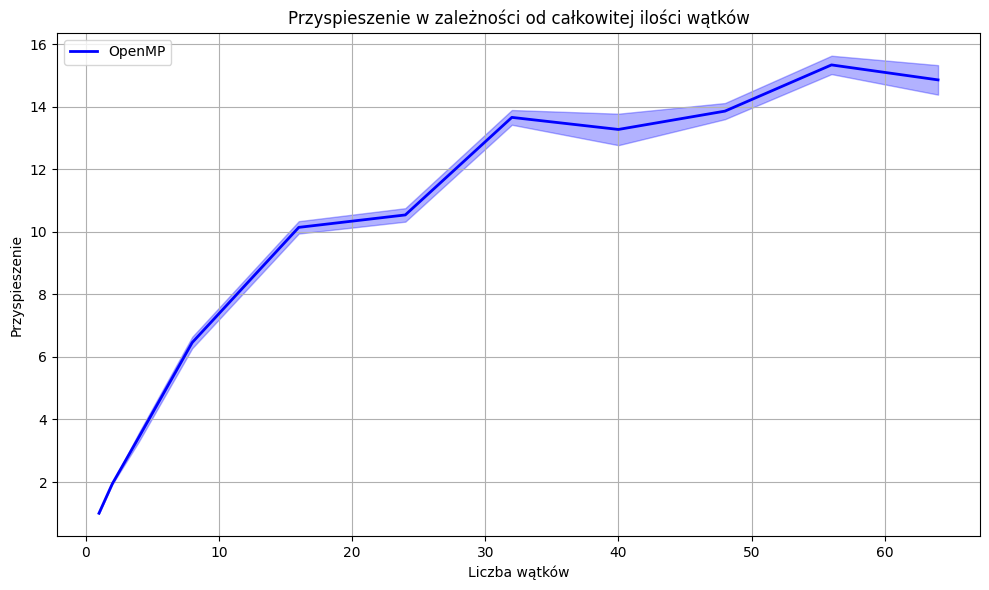
\includegraphics[width=0.8\textwidth]{openmp.png}
	\caption{Przyspieszenie dla OpenMP}
	\label{fig:openmp}
\end{figure}

\begin{figure}[h!]
	\centering
	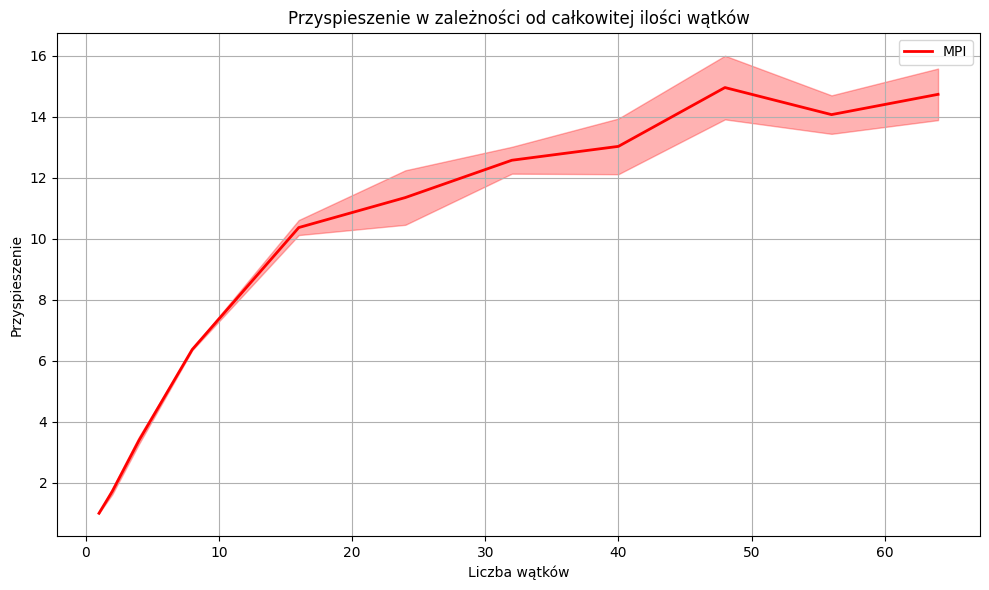
\includegraphics[width=0.8\textwidth]{mpi.png}
	\caption{Przyspieszenie dla MPI}
	\label{fig:mpi}
\end{figure}

\begin{figure}[h!]
	\centering
	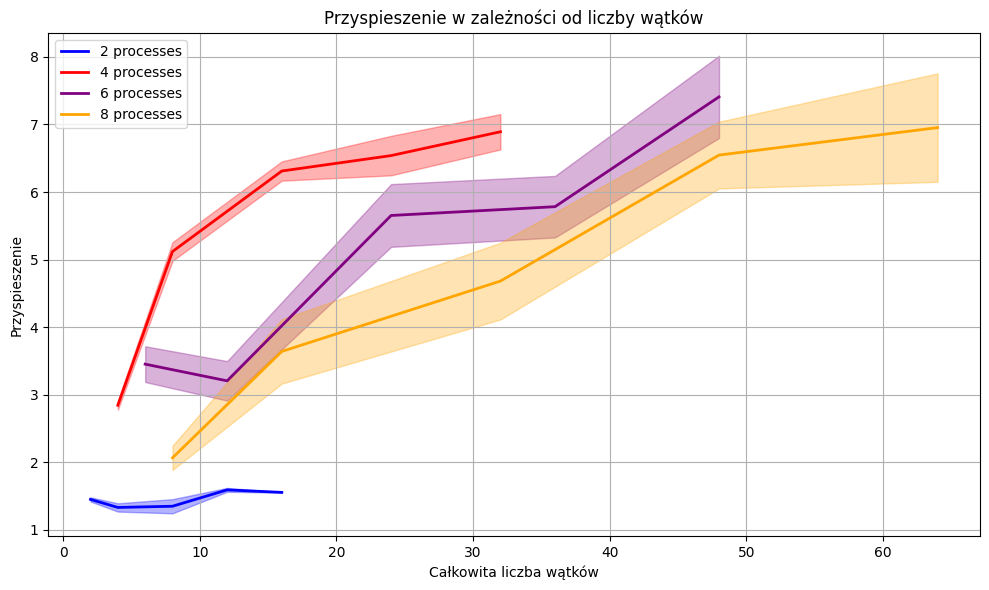
\includegraphics[width=0.8\textwidth]{mpi_openmp.png}
	\caption{Przyspieszenie dla MPI+OpenMP}
	\label{fig:mpi_openmp}
\end{figure}

\begin{figure}[h!]
	\centering
	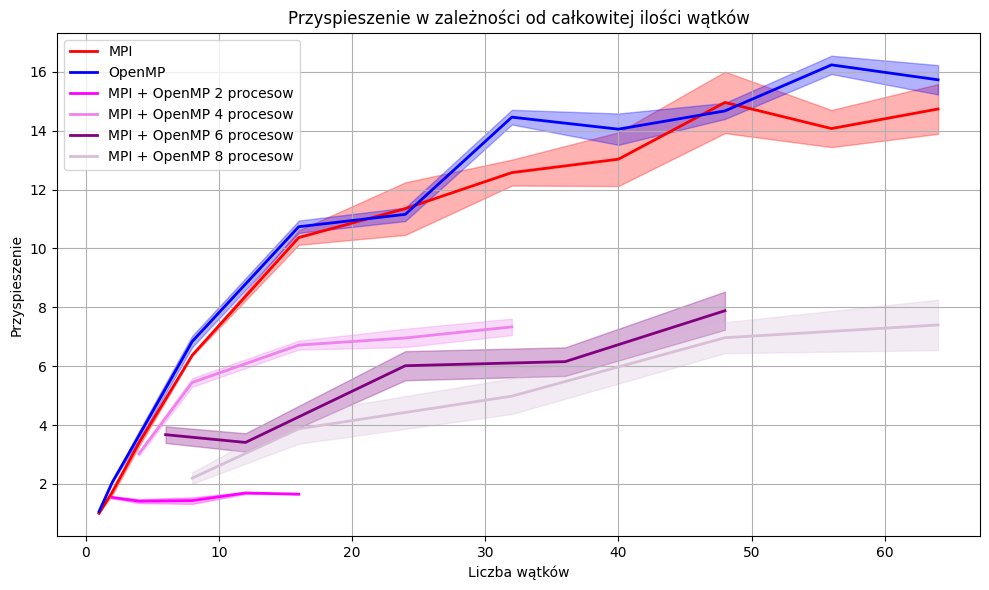
\includegraphics[width=0.8\textwidth]{all.png}
	\caption{Porównanie przyspieszeń dla wszystkich metod}
	\label{fig:all}
\end{figure}

\section{Wnioski}
Najlepsze wyniki uzyskały implementacje stosujące MPI lub OpenMP. 

Kombinacja MPI+OpenMP okazała się mniej wydajna ze względu na narzuty obu technologii, jednak umożliwia skalowanie algorytmu na wiele maszyn.

Dalsze optymalizacje mogą obejmować lepsze zarządzanie zasobami w konfiguracji MPI+OpenMP oraz dostosowanie wielkości partii przetwarzanych wiadomości.

\end{document}
